\documentclass[twoside,twocolumn, 10pt]{article}
\let\counterwithout\relax
\let\counterwithin\relax
\usepackage{chngcntr}

%\usepackage[sc]{fourier} % Use the Palatino font
\usepackage[T1]{fontenc} % Use 8-bit encoding that has 256 glyphs
\linespread{1.05} % Line spacing - Palatino needs more space between lines
\usepackage{microtype} % Slightly tweak font spacing for aesthetics

\usepackage[english]{babel} % Language hyphenation and typographical rules
\usepackage{blindtext}

\usepackage[hmarginratio=1:1,top=32mm,columnsep=20pt]{geometry} % Document margins
\usepackage[hang, small,labelfont=bf,up,textfont=it,up]{caption} % Custom captions under/above floats in tables or figures
\usepackage{booktabs} % Horizontal rules in tables

\usepackage{abstract} % Allows abstract customization
\renewcommand{\abstractnamefont}{\normalfont\bfseries} % Set the "Abstract" text to bold
\renewcommand{\abstracttextfont}{\normalfont\small\itshape} % Set the abstract itself to small italic text

\usepackage{todonotes}

\usepackage{titlesec} % Allows customization of titles
\titleformat{\section}[block]{\large\scshape\centering}{\thesection.}{1em}{} % Change the look of the section titles
\titleformat{\subsection}[block]{\large}{\thesubsection.}{1em}{} % Change the look of the section titles

\usepackage{fancyhdr} % Headers and footers
\pagestyle{fancy} % All pages have headers and footers
\fancyhead{} % Blank out the default header
\fancyfoot{} % Blank out the default footer
\fancyhead[C]{Computer Vision and Machine Learning $\bullet$ Spring 2019 $\bullet$ Aarhus University} % Custom header text
\fancyfoot[RO,LE]{\thepage} % Custom footer text

\usepackage{titling} % Customizing the title section

\usepackage[hidelinks]{hyperref} % For hyperlinks in the PDF

\usepackage{float}
\usepackage{amsmath}
\usepackage{amsfonts}
\usepackage{amssymb}
\usepackage{fancyhdr}
\usepackage{lastpage}
\usepackage{enumerate}
\usepackage{enumitem}
\setlist[enumerate]{noitemsep} % Make itemize lists more compact
\usepackage{graphicx}
\usepackage{pdfpages}
\usepackage{titlesec}
\usepackage{xcolor}
\usepackage[font={small},format=plain,labelfont={it,bf},justification=justified,singlelinecheck=false,labelsep=period]{caption}
\usepackage{subcaption}
\usepackage{titling}
\usepackage{listings,chngcntr}
%\usepackage{minted}
\usepackage{algorithm}
\usepackage{algpseudocode}
\usepackage{cleveref}
\usepackage{csquotes}
\usepackage{charter}
\usepackage{ltablex}
\usepackage{rotating}
\usepackage{booktabs}
\usepackage{pdflscape}
\usepackage[numbers]{natbib}


\renewcommand{\bibsection}{}
\bibliographystyle{IEEEtran}
\usepackage{multicol}
\raggedbottom
\usepackage{tabulary}

% ------------------------------------------------------------------------
% Restyle floats
% ------------------------------------------------------------------------


% ------------------------------------------------------------------------
% Fonts & colors
% ------------------------------------------------------------------------
% \setmainfont{Charter}
% \newfontfamily\aufont{AU Passata}
% \newenvironment{au}{\aufont}{\par}
\definecolor{AUDefault}{RGB}{0,61,133}

% ------------------------------------------------------------------------
% Algorithms & code
% ------------------------------------------------------------------------
\crefname{lstlisting}{listing}{listings}
\crefname{assumption}{assumption}{assumptions}
\crefname{algorithm}{algoritme}{algoritme}
\renewcommand{\algorithmicrequire}{\textbf{Input:}}
\renewcommand{\algorithmicensure}{\textbf{Output:}}
\makeatletter
\renewcommand*{\ALG@name}{Algorithm}
\makeatother

\definecolor{comm}{HTML}{2aa198}
\definecolor{keywrds}{HTML}{FF005A}
\definecolor{strng}{HTML}{DC143C}
\definecolor{back}{HTML}{1E1E1E}
\definecolor{light-gray}{gray}{0.95}
\definecolor{med-gray}{gray}{0.50}
\definecolor{dark-gray}{gray}{0.25}
\definecolor{dark-green}{HTML}{008000}
\lstdefinestyle{Txt}{ %
  backgroundcolor=\color{light-gray},
  basicstyle=\footnotesize\ttfamily\color{dark-gray},
  breakatwhitespace=false,
  breaklines=true,
  deletekeywords={...},
  escapeinside={\%*}{*)},
  extendedchars=true,
  frame=bt,
  numbers=left,
  numbersep=5pt,
  numberstyle=\tiny\color{gray},
  showspaces=false,
  showstringspaces=false,
  showtabs=false,
  tabsize=2,
}
\lstdefinestyle{Python}{ %
  backgroundcolor=\color{light-gray},
  basicstyle=\footnotesize\ttfamily\color{dark-gray},
  breakatwhitespace=false,
  breaklines=true,
  commentstyle=\color{med-gray},
  deletekeywords={...},
  escapeinside={\%*}{*)},
  extendedchars=true,
  frame=bt,
  keepspaces=true,
  keywordstyle=\color{dark-green},
  language=Python,
  %otherkeywords={1, 2, 3, 4, 5, 6, 7, 8 ,9 , 0, -, =, +, :, *, !}, ,
  numbers=left,
  numbersep=5pt,
  numberstyle=\tiny\color{gray},
  showspaces=false,
  showstringspaces=false,
  showtabs=false,
  stringstyle=\color{strng},
  tabsize=2,
}

% ------------------------------------------------------------------------
% Counters, lists
% ------------------------------------------------------------------------
\setcounter{secnumdepth}{3}
\setcounter{tocdepth}{2}
\numberwithin{figure}{section}
\numberwithin{table}{section}
\numberwithin{equation}{section}
\numberwithin{algorithm}{section}
\setlist[itemize]{noitemsep}
%----------------------------------------------------------------------------------------
%	TITLE SECTION
%----------------------------------------------------------------------------------------

\setlength{\droptitle}{-4\baselineskip} % Move the title up

\pretitle{\begin{center}\Huge\bfseries} % Article title formatting
\posttitle{\end{center}} % Article title closing formatting
\title{Image Classification of Aquatic Macroinvertebrates} % Article title
\author{%
\textsc{Alex Justesen Karlsen} \\
\normalsize Aarhus University - Department of Engineering\\ % Your institution
\normalsize \href{mailto:au515295@post.au.dk}{au515295@post.au.dk} % Your email address
}
\date{\today} % Leave empty to omit a date
\renewcommand{\maketitlehookd}{%
\begin{abstract}
\noindent The paper documents my work on the in-class Kaggle Challenge; 'AU-ENG-CVML2019'. The paper is a mandatory submission in the Computer Vision and Machine Learning 2019 course at Aarhus University. The machine learning challenge is to obtain better classification result on th FIN-Benthic dataset of 29 classes of aquatic macroinvertebrates. The paper explains the dataset and a way to augment the dataset to gain better results. Furthermore the paper describes the machine learning methods used and the results.
\end{abstract}
}

%----------------------------------------------------------------------------------------

\begin{document}

% Print the title
\maketitle

%----------------------------------------------------------------------------------------
%	ARTICLE CONTENTS
%----------------------------------------------------------------------------------------

\section{Introduction} \label{sec:introduction}
Life below water is a critical ecosystem, that experiences a lot of challenging changes. It so important a challenge, that it has found its' way to the UN Sustainable Goals \cite{UN}. The Finnish Environment Institute \cite{meissner} SYKE claims, that the loss of aquatic biodiversity and associated Ecosystem Services is one of the most pressing problems on Earth. SYKE launched the DETECT project \cite{DETECT}, which aims to identify the various species of aquatic macroinvertebrates by imagery and classification using computer vision and machine learning. \\

This paper is a part of the Computer Vision and Machine Learning course at Aarhus University. It documnets my work on solving the in-class Kaggle Challenge. The aim of the Kaggle challenge is improving the classification accuracy of classifiyng the 29 classes of aquaitc macroinvertebrates. Machine Learning and state-of-the-art Deep Learning approaches utilizing Convolutional Neural Networks, are used to examine the different methods and get hand-on experience with a real classification challenge. \\

The rest of the paper is structured as follows; section \ref{sec:dataset} desribes the data set in more depth and how the structure specific structure of the dataset have been used to improve the accuracy. Section \ref{sec:methods} describes the machine learning and deep learning methods used in the project. Section \ref{sec:results} describes and discusses the results obtained from applying the methods. Section \ref{sec:discussion} is a discussion of the overall results and lastly in section \ref{sec:conclusion} the project is concluded upon.

%------------------------------------------------
\section{Data Set} \label{sec:dataset}
The FIN-Benthic \cite{finbenthic} dataset 2 are used in this paper. The dataset consists of 29 different classes of aquatic macroinvertebrates. 

\begin{figure}[H]
    \centering
    \includegraphics[width=0.35\textwidth]{figures/bugs.png}
    \caption{Example of aquatic macroinvertebrates}
\end{figure}

The datset counts 11,588 images divided into training set (5830 images), validation set (2298 images) and test set (3460 images). The training and validation set are annotated with class labels, whereas the test set are not. This paper is a part of a Kaggle\footnote{Kaggle is an online community of data scientists and machine learners. Red more: https://www.kaggle.com/getting-started/44916}Challenge with the aim of getting the best classification score on the test set, that are evaluated on Kaggle. For the challenge feature vectors produced by an AlexNet\cite{Krizhevsky:2012} trained on the raw images. The features are the output of the last convolutional layer and flattened into a one-dimnesional vector with 4096 features. All images and vectors comes in pairs of images of the same bug taken form perpendicular angles, an attempt to take advantage of the systematic series the images are all images vertically stacked. If we have a pair of $x_1$ and $x_2$, then $x_1$ and $x_2$ are stacked as a combination of the two; 

$$x_1=\begin{bmatrix} x_{1} \\ x_{2} \\ \end{bmatrix}, x_2 = \begin{bmatrix} x_{2} \\ x_{1} \\ \end{bmatrix}$$

The vectors now contains $2 \times 4096 = 8192$ features. The concatenated version of the dataset are referred to as FIN-Benthic-Concatenated. Futhermore the training and validation sets are merged to form a combined set, to enable Cross-Validation for the different classification algorithms tested in this paper. Cross-Validation and Machine Learning methods used are described in the next section.

%------------------------------------------------
\section{Methods} \label{sec:methods}
Several experiments on this supervised learning challenge have been conducted using a variety of different techniques for classification are peformed on the two encoded datasets; FIN-Benthic and FIN-Benthic-concatenated. The classification methods are; k-Nearest Neighbors (kNN), Linear Discriminant Analysis (LDA), Support Vector Machines (SVM), Perceptron and Neural Networks (NN). Commonly for all these supervised learning algorithm is the need for training. Training an algorithm is an optimization process of a function and a loss criterion, that explains the goodness of the model as training progresses until convergence. Cross Validation (CV) are use for model selection to evaluate the best performing model. All the methods have been applied to the datasets on full dimensions and additionally with dimensionality reduction as a preprocessing step in the classification pipeline. Grid search have been used to search for good hyperparameters. Hyperparameters are user specified parameter to control the algorithms behaviour \cite{Goodfellow-et-al-2016}. Hyper parameter search have been applied for all classifiers. Furthermore the degree of dimensionality reduction have been investigated in the same manner. Lastly existing Convolutional Neural Network architectures have been used on the raw images and using the promise of transfer learning to use a pretrained model to gain faster and better performing models on small datasets. For the transfer learning task the existing train, validation and test split have been used.

\paragraph{k-Nearest Neighbors (kNN)}

K-Nearest Neighbor is a distance-based classifier and as the name implies, classifies to the most common occuring class of the k-nearest neighbors \cite{karpathy}. There exist a variety of distance metrics, some example are; euclidean, minikowski and manhattan distance \cite{AIML}. 

\begin{figure}[H]
    \centering
    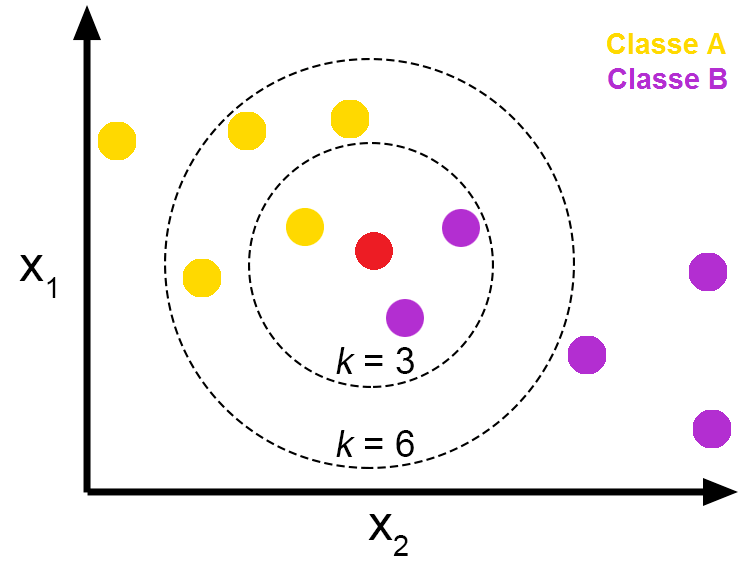
\includegraphics[width=0.4\textwidth]{figures/knn.png}
    \caption[]{k-Nearest Neighbor classifies the red sample to class B for $k=3$, however for $k=6$ it classifies to class A. Credits: Italo José}
    \label{fig:knn}
\end{figure}

\paragraph{Linear Discrmininat Analysis (LDA)}

Linear Discrmininat Analysis is a linear transformation of the data. The linear transformation is an optimization, that tries to maximize the distance between classes and minimize the distance within a class\cite{AIML}. Figure \ref{fig:lda_dec} shows how LDA discriminates two classes.

\begin{figure}[H]
    \centering
    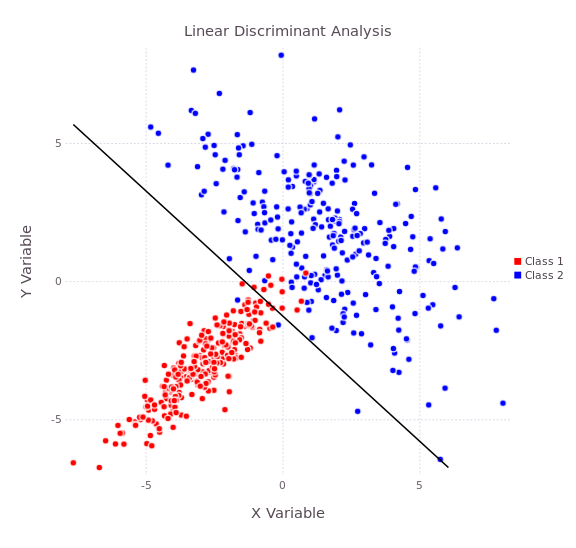
\includegraphics[width=0.4\textwidth]{figures/lda_deci.png}
    \caption[]{LDA creates a linear decision function. The linear decision function is a decision hyperplane, which discriminates classes. Credits: Tim Thatcher}
    \label{fig:lda_dec}
\end{figure}

LDA can also be used for dimensionality reduction, this would be further explained later.

\paragraph{Support Vector Machine (SVM)}

SVM can be used for classification. SVM tries to find the decision hyperplanes, that maximizes th distance between classes \cite{IR}. The decision hyperplane are given by a linear function $w^Tx+b$, when the function is positive it predicts th class to be present, and intuitively the class is not present, when the function is negative \cite{Goodfellow-et-al-2016}. The Support Vector Machine uses support vectors to define the decision hyperplane. The support vectors are vectors of the training data, that maximizes the margin between to classes. The original SVM proposed by Boser et al. \cite{Boser} utilize a hard-margin. The hard-margin is the optimal decision hyperplane, however it only works well when the data is linearly seperable. Vapnik et al. \cite{Vapnik} proposed a soft-margin, which is more robust to noise by introducing some slack by introducing the hinge loss function.

One of the most promising contribution associated with SVMs is the kernel trick. The kernel trick makes not only SVM useful even when data is not linearly seperable, but all machine learning algorithms, that can be rewritten exclusively in terms of dot product between examples. The kernel trick is a mapping of the data into a higher dimensional space - even with indefinite dimensions. The kernel trick is equivalent to transforming all data points into higher dimensions, but with a lot less computational demands. In the high dimensional space a linear decision boundary can be obtained. One of the most widely used kernel is the gaussian kernel or radial basis function (RBF), which maps to an indefinite dimensional space \cite{Goodfellow-et-al-2016}.

\begin{figure}[H]
    \centering
    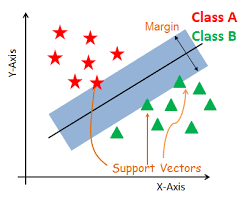
\includegraphics[width=0.4\textwidth]{figures/svm.png}
    \caption[]{A binary SVM constructing the decision hyperplane, that maximizes the margin between the support vectors of the two classes. Credits: Avinash Navlani}
    \label{fig:svm}
\end{figure}

\paragraph{Perceptron}

Perceptrons is a single layer Neural Network. The perceptron was set forth by Frank RosenBlatt \cite{Perceptron}, as a way of mimicking human perception. Perceptrons produces a linear decision function and only performs well on linearly seperable data. 

\begin{figure}[H]
    \centering
    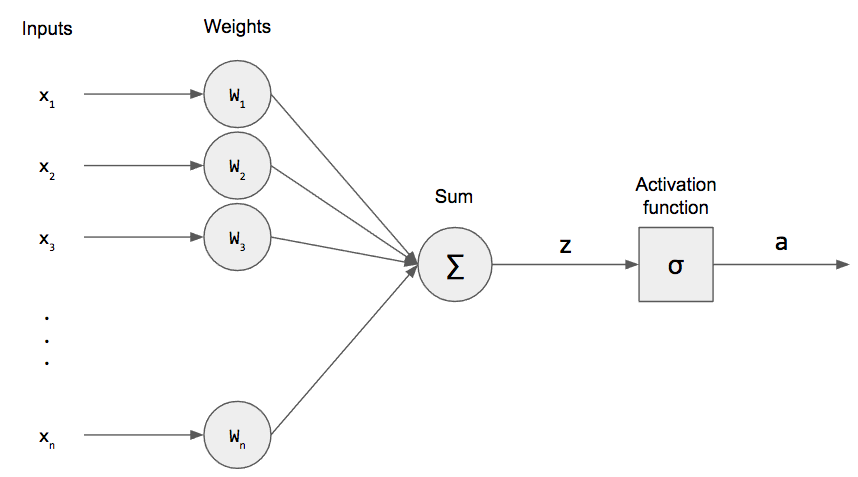
\includegraphics[width=0.4\textwidth]{figures/perceptron.png}
    \caption[]{The perceptron takes a feature vector as input. All the feature are multiplied by a weight. The weight are then summed to what is called a weighted sum. An activation function are applied to the weighted sum. The output of the activation function is the classification. Credits: Stanley Obumneme Dukor}
    \label{fig:perc}
\end{figure}

The perceptron are trained by iteratively updating the weights to produce the correct output for the training data. The loss function are rather simple, if the sample is correctly classified th loss function will output zero and it will output 1 if misclassified. This means the perceptron's weight are only updated when is fails to classify a sample. 

\paragraph{Neural Network (NN)}

Neural Networks extends the perceptron. This ideas was sparked by progress within biology mapping human cognition into a network of perceptrons i.e. neurons. The work working Aritifical Neural Network was completed by A. G. Ivakhnenko and V. G. Lapa \cite{Alexey}. The perceptrons where extended by adding more layers between input and output referred to as hidden layers. The NN produces non-linear decision functions, thus overcomes the short comming of the perceptron.  

\begin{figure}[H]
    \centering
    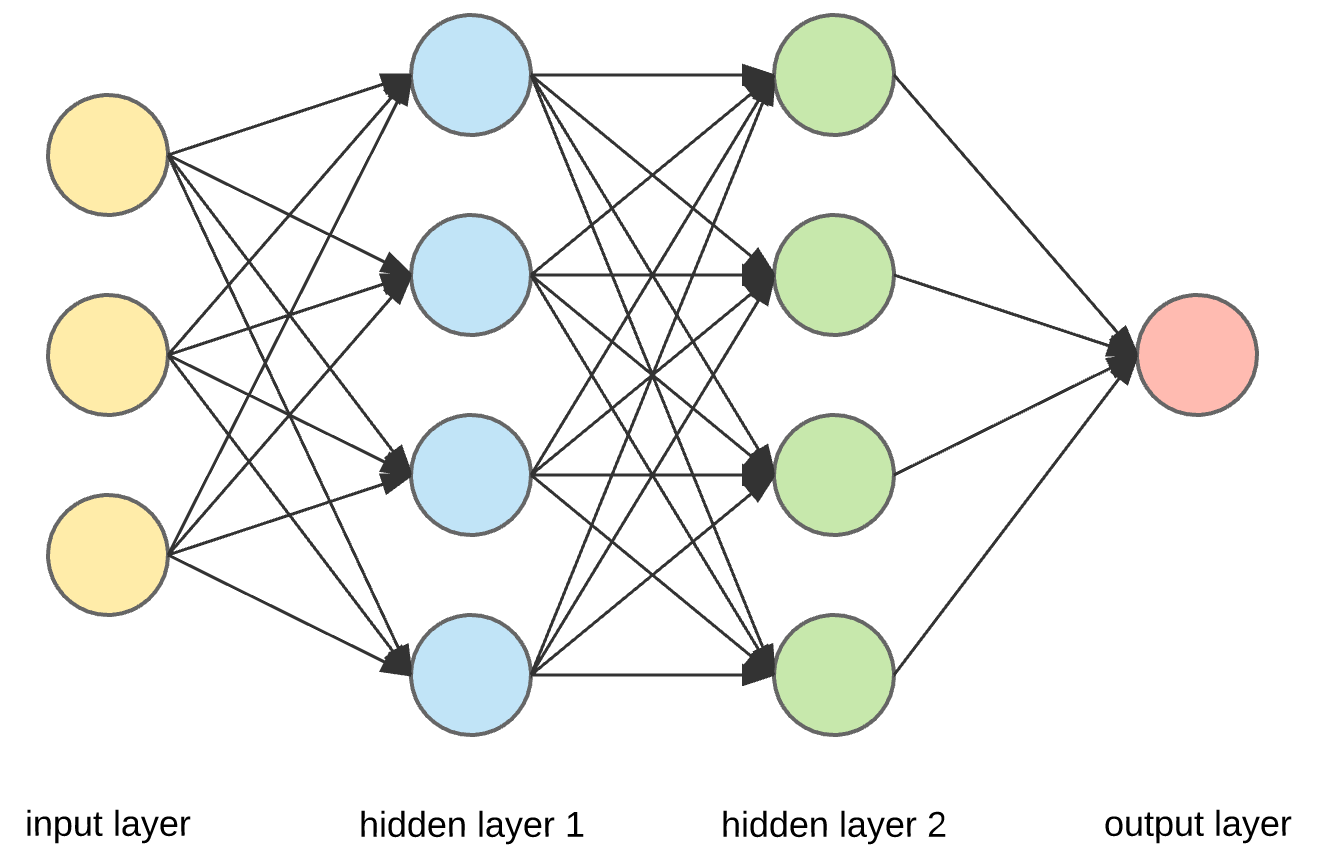
\includegraphics[width=0.4\textwidth]{figures/nn.png}
    \caption[]{Neural Network with two hidden layers and each layer is fomred by a number of neurons. A fully-connected dense neural network receives all output from previous layer as input. The input are multiplied by the neuron's weight and adding bias. At last the non-linear acitvation function is applied. Credits: Arden Dertat}
    \label{fig:nn}
\end{figure}

Training a NN is way more complex than a perceptron. The training are done using feedforward and back-propagation. Training vectors are given to the network, where all nodes do their operations upon receiving and ninput anf feeding it forward to the next layer, when it reaches the end of the network and error term is computed using the loss function. The error are then backpropagted. throuout the network, where the nodes' contribution to the error is computed. Using gradients the network weight are optimized. 

\paragraph{Convolutional Neural Network (CNN)}

\paragraph{Dimensionality Reduction}

Dimensionality reduction as the name implies downscales the feature space into a lower dimnesional space. The techniques used in this paper is the already covered LDA and Principal Component Analysis (PCA).

\subparagraph{Principal Component Analysis (PCA)}

PCA is an unsupervised leraning technique. It learns an othogonal linear transformation onto a smaller feature space. The number of dimensions i.e. principal components are a hyperparameter. PCA tries to preserve as much as the information i.e. variance as possible. The first component i.e. dimension is a projection a long the axis of the data with the variance, the second component orthogoanl to the first axi. Th second compoent descirbes the axis with second most variance. The third the third most variance and so on, as the figure \ref{fig:pca} shows.

\begin{figure}[H]
    \centering
    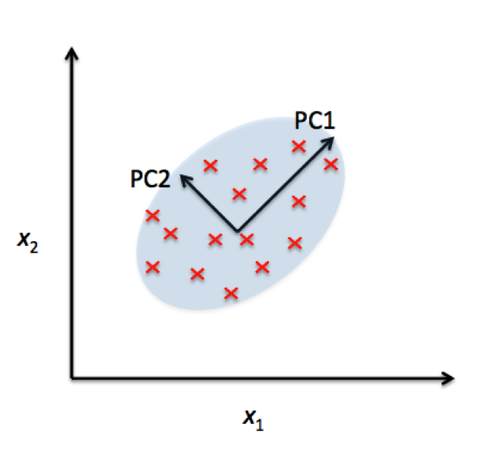
\includegraphics[width=0.4\textwidth]{figures/pca.png}
    \caption[]{Principal Component Analysis in a 2 dimensional space. PCA rotates the data to be perpendicular to the principal components axises. Credits: Sebastian Raschka}
    \label{fig:pca}
\end{figure}

\subparagraph{Linear Discriminant Analysis (LDA)}
As mention LDA can be used for dimensionality reduction as well. One must specify the $n$ number of components i.e. dimensions to transform the data onto, if the $n$ are less than the original data's dimensions D, the the number of dimensions will be reduced. 

\begin{figure}[H]
    \centering
    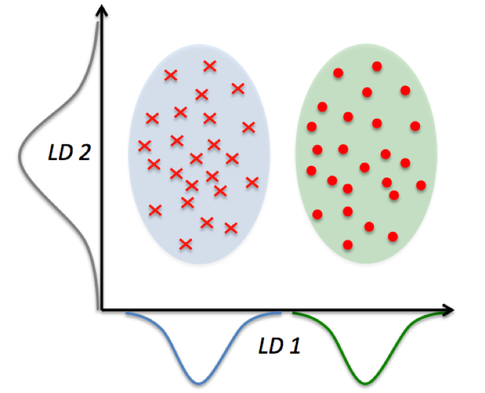
\includegraphics[width=0.4\textwidth]{figures/lda.png}
    \caption[]{Linear Discriminant Analysis project the data onto and axis, that maximize the distance between the classes and minimizes the distance within the respective classes. Credits: Sebastian Raschka}
    \label{fig:lda}
\end{figure}

\paragraph{Model Selection}

Model selection are procedures to train the best model and avoid overfitting the model to the training data. Overfitting is the pitfall of having a model, that desribes the training data too well, thus suffers to not generalising the true underlying structure of the data. Although other methods exists the two used in the paper are Validation Holdout and Cross Validation. 

\subparagraph{Validation Holdout}

Validation Holdout takes a fraction of your available labelled data and hold it out of the training procedure. 

\begin{figure}[H]
    \centering
    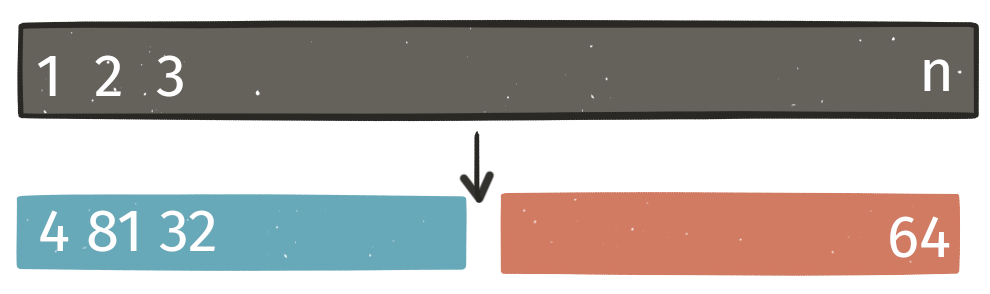
\includegraphics[width=0.4\textwidth]{figures/validationset.png}
    \caption[]{The validation subset is then used to validate the model's performance on data it has not been training.}
    \label{fig:val_holdout}
\end{figure}

The assumption is, that the holdout set resembles the true data, since it has been drawn from the same distribution \cite{Goodfellow-et-al-2016}. If the model performs well on both training and validation it is assumed to be a good model. The split is typically made 70/30 for training data and validation data respectively. 

\subparagraph{Cross Validation (CV)}

Cross Validation extends on the holdout validation. $k$-fold Cross Validation create $k$ experiments compared to one. The entire data set are split in $k$ folds, for every $k$ step one subset is for validation and the remaining $k-1$ fold are used for training \cite{Goodfellow-et-al-2016}. Figure \ref{fig:cv} illustrates the idea. 

\begin{figure}[H]
    \centering
    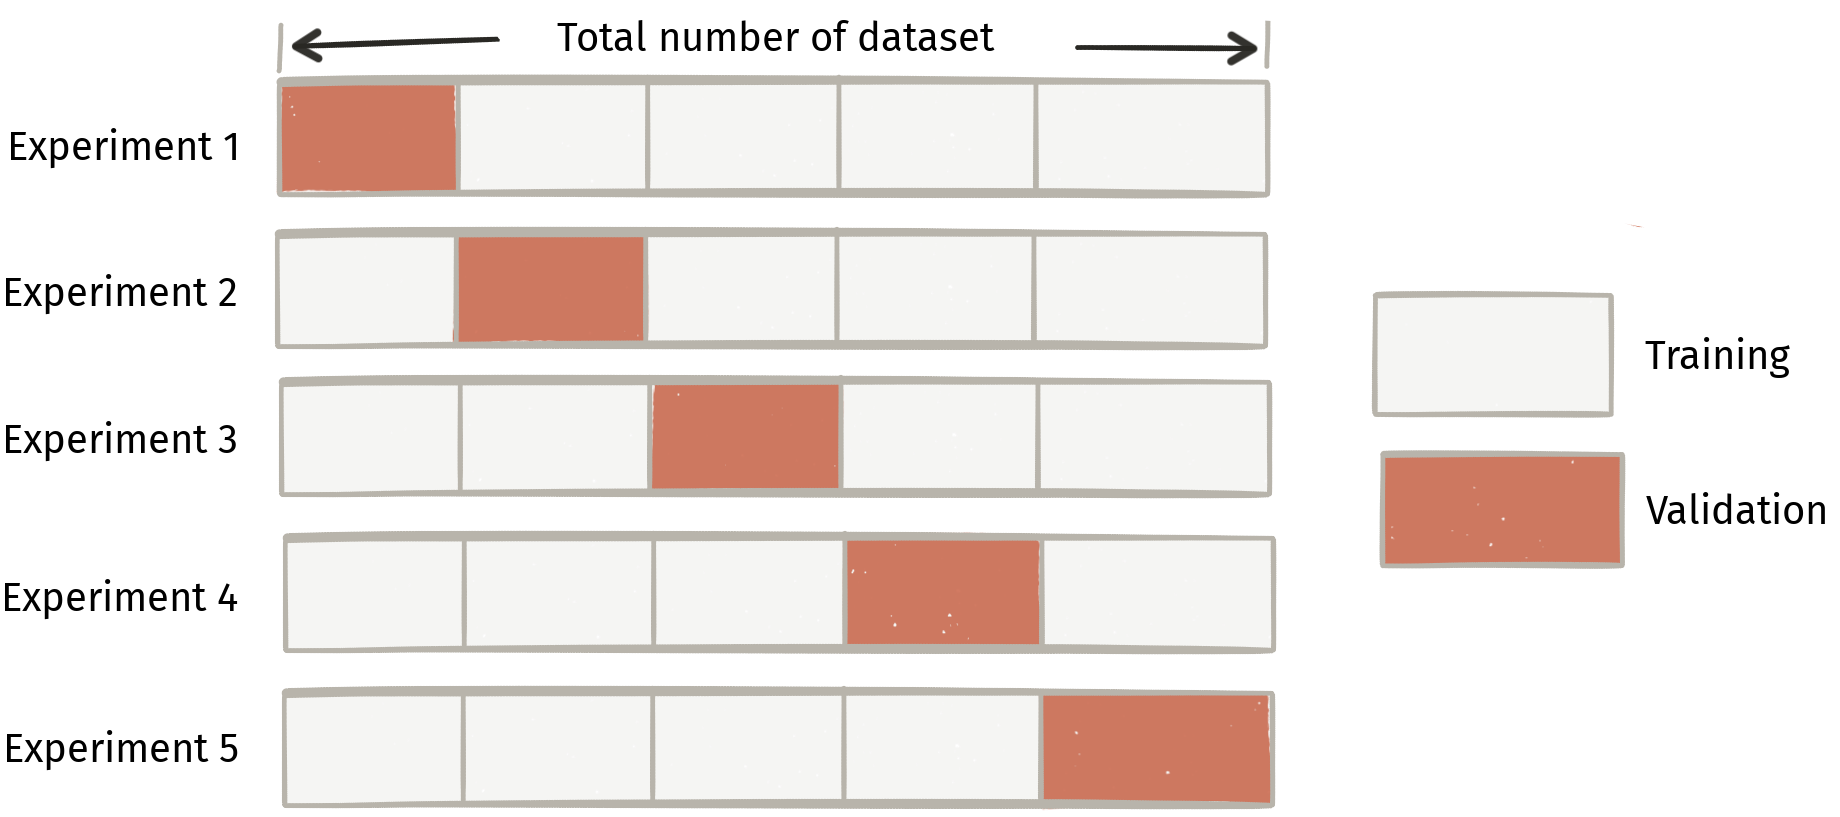
\includegraphics[width=0.5\textwidth]{figures/cv.png}
    \caption[]{Cross Validation ensures that the model have been trained on all the data and validated as well. The selection folds are typically either $k=5$ or $k=10$. }
    \label{fig:cv}
\end{figure}

\paragraph{Hyperparameter Search}

There are mainly two approaches to search for hyperparameters; Random Search and Grid Search other than heuristic guessing. In this paper Grid Search are used.

\subparagraph{Grid Search}

Grid Search is an approach to seek better hyperparameters for your model. You specify a set of options for all hyperparameters and then seacrh all possible combination in the grid. 

\begin{figure}[H]
    \centering
    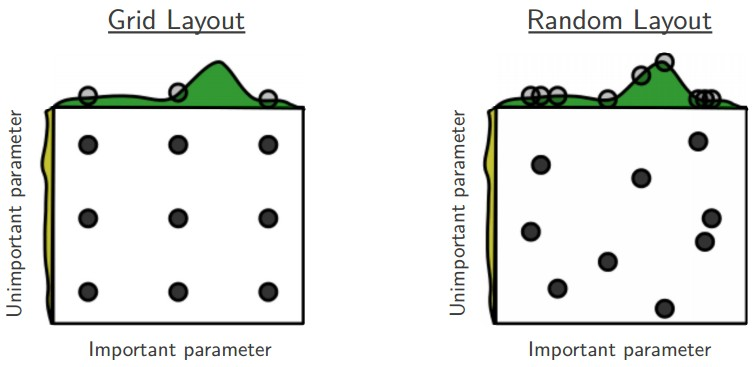
\includegraphics[width=0.4\textwidth]{figures/gridsearch_vs_randomsearch.jpeg}
    \caption[]{Grid search is a systematic approach to explore a broader space of hyperparameters although at the cost of additional time. The down-side of this approch is, that it is still based on intuition of good hyperparameters. The random approach are also widely used and might be preffered, as it may find a sweet spot, that goes beyond human intuition, however that is no guarantee, and it is still time costly \cite{Bergstra}. Credits: Bergstra and Bengio}
    \label{fig:gs_vs_rs}
\end{figure}

  

%------------------------------------------------

\section{Results} \label{sec:results}
Two main experiments have been conducted; the first experiment involves applying the aforementioned machine learning methods on the feature extracted vector. The second experiment involves applying deep learning practices on the raw image data. 

\subsection*{Experiment 1: Machine Learning}
The machine learning experiments are implemented in Python 3 using the SciKit Learn library, except the Neural Network that are implemented in Keras using Tensorflow backend. \\

All classifiers have been run on the FIN-Benthic dataset and on the FIN-Benthic concatenated dataset using Grid Search and CV to find the best hyperparameters, except the neural networks. As grid search has been used to find the best set of parameters for each of the classifiers and on the different datasets, it has not given the same results for best hyperparameter settings. Only the best performing setting of hyperparameters for each classifier are presented in this paper.

\begin{figure}[H]
    \centering
    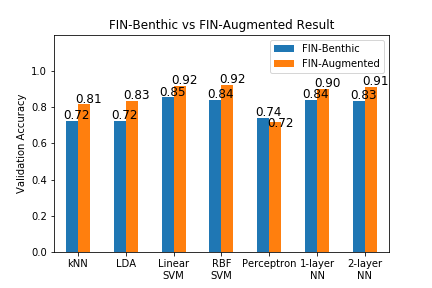
\includegraphics[width=0.5\textwidth]{figures/fin-benthic-same.png}
    \caption[]{The best setting for each of the classifiers in terms of accuracy. Generally the classifiers perform best on the concatenated dataset. The assumption about concatenating the pair sample of the same bug holds true.}
    \label{fig:fin_ben_concat}
\end{figure}

I added PCA to the classification pipeline and ran the same grid search on all the classifiers on both datasets. For all runs the dimensionality have been reduced to $n=\{128, 256, 512, 1024\}$ principal components. PCA add additional time to the pipeline, however the time to train and predict on fewer dimensions significantly improved. Altough the dimensionality have been reduced with a large margin it does not have huge impact on the classification accuracy.

\todo{Bring some results using dimensionality reduction}

\subsection*{Experiment 2: Deep Learning}

% \subparagraph{k-Nearest Neigbor}

% The grid for kNN parameters was the $k$ number of neighbors; $k=\{1, 5, 10\}$. The tedency was a higher training accuracy with lower $k$ and higher validation score with higher $k$. This indicates the data is not well clustered in classes. $k=10$ was the best performing in terms of mean cross validation score with an accuracy of $0.72$.

% \subparagraph{Linear Discriminant Analysis}

% The grid for LDA was the $n$ number of components; $n = \{64, 128, 256\}$. All setting had exactly same performance of validation accuracy $0.72$ and $1.00$ on the training data.  

% \subparagraph{Support Vector Machine}

% The grid for SVM was both the $C = \{0.1, 1, 10\}$ value and the $kernel = \{'linear', 'rbf'\}$. $C$ is the penalty term, a lower $C$ gives a softer margin, whereas a higher value gives a harder margin. The kernel using a linear SVM or using the kernel trick with an Radial Basis Function kernel. 

% \subparagraph{Perceptron}

% The p




%------------------------------------------------

\section{Discussion} \label{sec:discussion}
Taking advantage of the pairwise structure of the FIN-Benthic data set significantly improves the machine learning algorithm's classification performance. The double amount of information seems very useful and can be backed up by looking at the raw images. In most cases the images resembles each other, however there are cases, where the images seems to be taken from an unfortunate angle. The doubled information seems to handle this problem. Nonetheless inspecting the predicted class labels, one can see, that they are still not completely pairwise segmented. A postprocessing step if using a probabilistic classification model can be proposed. Summing the outcome of class probabilities for the pair and classify to the most probable for the pair could be advantageous.

A future step is to look at random search instead grid search. Although improvements where found using grid search and I started with coarse grids and narrowed down the search space using finer grid, there might be combinations, that I did not consider and which could have given better results. 

I have tested out a set of different classification method and the best performing seems to be Support Vector Machines and Fully-Connected Neural Network for the vectorized AlexNet features. It would have been interesting to train a state-of-the-art CNN over a long period of time, to see if the features from such a network would in fact improve the features, thus gives a better accuracy for all the methods. Nowadays architectures like GoogleNetV4 accuracy of 0.803 on the ImageNet data set\cite{SzegedyIV16}, which have the size required to train such deep models. Transfer learning reuses the weights from e.g. ImageNet to solve a another classification task. The model can be fine-tuned to better fit the special cases of the new data set. 

%------------------------------------------------

\section{Conclusion} \label{sec:conclusion}
I have gained a lot of experience with a practical machine learning challenge. I used the pair-wise information in the data set to optimize model accuracy to a $0.92$ validation accuracy and $\approx 0.86$ test accuracy on the Kaggle Challenge's test set. I struggled with deep learning performance and did not have the resources to overcome the challenges. 

%----------------------------------------------------------------------------------------
%	REFERENCE LIST
%----------------------------------------------------------------------------------------
\section*{References}
\bibliography{content/bibliography}
\input{content/appendix.tex}
%----------------------------------------------------------------------------------------

\end{document}
